\chapter{Abstract and Summary}\label{Ch1_AbstractAndAcknowledgements}

\section{Acknowledgements}

I would to thank my supervisor Prof. David Jordan for his invaluable support and guidance throughout the project;
Christopher Butler for providing the TeX code so I could easily set up the blueprint, and hopefully, improve and add to his amazing exposition of
\textbf{Dickson's Classification Theorem} \cite{butler}.

I would also like to thank Prof. Kevin Buzzard for his support, patience and guidance throughout the project. His advice and comments on how I should go about formalising mathematics have been of utmost value. 

Finally, I would like to thank the many members of the Lean Zulip community who have provided insightful ideas and comments that have helped me progress much faster than otherwise, 
this also includes assistance with technical issues with setting up the blueprint and so forth. I am grateful to:

\begin{itemize}
    \item Artie Khovanov
    \item David Loeffler
    \item Mitchell Lee
    \item Yakov Pechersky
    \item Edward van de Meent
    \item Ruben Van de Velde
    \item Andrew Yang
    \item Patrick Massot
    \item Johan Commelin
    \item Scott Carnahan
    \item Damiano Testa
    \item Aron Liu
\end{itemize}

I apologise if I have forgotten to include any names.

\section{Summary}

The primary aim of this project is to present the ongoing formalisation of the classification of finite subgroups of $\PGL_2(\Fbar_p)$ in the Lean proof assistant. This result fits into to the much larger and more ambitious project
of formalising Fermat's Last Theorem \href{https://imperialcollegelondon.github.io/FLT/blueprint/}{FLT} in Lean, an effort being led by Prof. Kevin Buzzard at Imperial College London. In fact, this theorem corresponds to theorem 12.7 in \href{https://imperialcollegelondon.github.io/FLT/blueprint/ch_bestiary.html}{Appendix}.
Furthermore, another goal of this project is to serve as a Rosetta stone for how informal mathematics corresponds to formal mathematics; the hope is that the blueprint will serve as an example of how late undergraduate mathematics is formalised using \texttt{mathlib}, the mathematics library of Lean.
A pleasant outcome of presenting both the informal and formal mathematics alongside into one cohesive website is that it allows to new ways of presenting mathematics, where the informal and formal mathematics complement each other.


\section{How to read this blueprint}

The general layout of the blueprint is:

\begin{enumerate}
    \item Statement of Definition/Theorem/Lemma/Corollary
    \item Proof where relevant.
    \item Formalisation of the statement of the Definition/Theorem/Lemma/Corollary
    and proof.
    \item Further remarks on the formalisation where relevant.
\end{enumerate}
\subsection{Navigating the blueprint}

The main distinctions are due to the interactive side of this blueprint:

\begin{itemize}
    \item In the bottom right corner there should a subset of the following buttons: 
        \begin{enumerate}
            \item Eye-minus $\boxdot^-$: Will toggle the blueprint to display less text.
            \item Eye-plus $\boxdot^+$: Will toggle the blueprint to display more text. 
            \item Arrow-left $\Leftarrow$: Will navigate the page to the previous chapter
            \item Arrow-up $\Uparrow$: Will navigate the page to the index.
            \item Arrow-right $\Rightarrow$: Will navigate to the next chapter.
        \end{enumerate}
\end{itemize}

\textbf{Important note}

There are three states for toggling how much text, ordered from least to most text being displayed.

\begin{enumerate}
    \item Displays only definitions and statements of theorems.
    \item Displays definitions, statements, accompanying text and allows to toggle proofs being displayed or being hidden always.
    \item Displays defintions, statements, accompanying text and proofs.
\end{enumerate}

\subsection{Note on \texttt{remarks}}

Any content that is within the \texttt{remark}, that is anything within a box like:

\begin{remark}[A remark]
    Content of remark
\end{remark}

environment will be dedicated towards explaining or illustrating how the mathematics formalised in Lean might differ to 
how the informal mathematics is often presented, may often omit implicit details, or how \texttt{mathlib} or myself have come up with particular
abstractions which ease the process of formalisation.

\subsubsection{The dependency graph}

To the left of the website there should be an index which lists out the chapters of this blueprint which will eventually contain all proofs and intermediate formal statements necessary
to prove the overarching claim. But, in addition to the index of chapters and bibliography there is an entry for the \texttt{Dependency graph}.

This will display a directed acyclic graph which demonstrates how all relevant definitions and statements feed into each to produce the final claim.

\textbf{Note} the dependency graph and icons to the bottom right are only visible if the html page is launched on a local server since
having otherwise would be a security hazard.

If the reader wishes to see the dependency graph and the icons (the icons are still functional despite not being visible), the reader should run
\texttt{python3 -m http.server} within the folder which contains the HTML for these pages (assumes a python installation).

\begin{figure}
    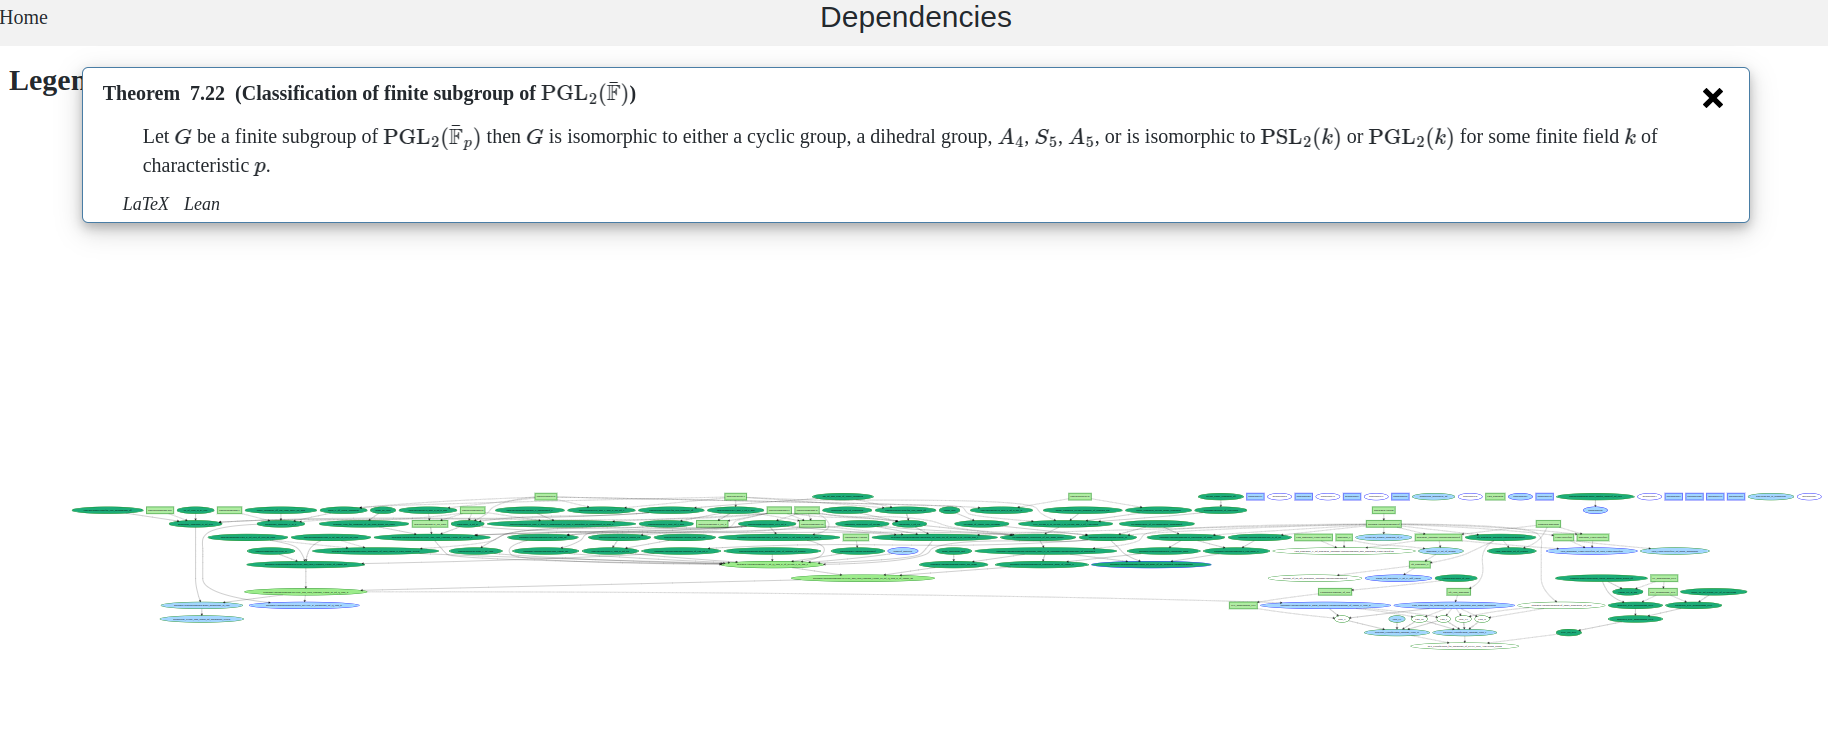
\includegraphics[width=0.8\textwidth]{dependencygraph.png}
\end{figure}

\subsection{Distinguishing my work from Christopher Butler's work}


Naturally, the largest bulk of my original work in this project consists of the formalisation of mathematics since Christopher Butler has kindly provided the TeX for his original master's thesis exposition on
the classification of finite subgroups of $\SL_2(F)$. Bear in mind, the goal of the formalisation is this classification of finite subgroups of $\PGL_2(\Fbar)$, it turns out the classifications problems are tightly
related and this is why a lot of Christopher Butler's work is reused here.

Nonetheless, it may be surprising to understand that so far, around two thirds of the exposition alongside additional results relevant to concrete goal for formalising Fermat's Last Theorem have been formalised.

It turns out, that so far there is a rough correspondence for two lines of code/formal mathematics per one line of informal/pen-and-paper mathematics. That is to say, if 50 lines of code were displayed per page, all
the code written would constitute a total of around 86 pages, since there are 4344 lines of Lean.

Moreover, on the basis of academic integrity I provide a rough overview of what constitutes my work and what constitutes Christopher Butler's work.

\begin{itemize}
    \item My work:
    
    All the \texttt{verbatim} environments which contain Lean code is my original contribution.
    
    Chapter 2 and Chapter 4 constitute my work completely; a lot of the structure and set up for Chapter 6 is my work
    since the original argument turned out to be not easily formalisable; Chapter 5 includes many intermediate lemmas relevant
    to the classification of elements of $\SL_2(F)$ up to conjugation.


    \item Christopher Butler's work:
    
    Aside from the Lean code displayed in Chapter 3 and Chapter 7, these chapters are primarily Christopher Butler's work. Aside from
    when the embedding of $\mathbb{F}_{p^n}$ into $\mathbb{F}_{p^{2n}}$ and the group presentation for the dihedral group were defined 
    in Chapter 7.
    
    Aside from particular points where I have completely modified the approach to prove a particular statement, most proofs belong to Christopher Butler's exposition.
    
    Part of the intention of this is to highlight how the formal proof differs from the 
    original informal proof; I have tried at every stage to follow the argument within Christopher Butler's exposition. 
    
    Therefore, it is the hope that comparing the informal and formal mathematics side by side should be interesting to the reader.

    There are parts where the arguments have had to stray from the original path:
    
    \begin{itemize}
        \item When classifying elements of $\SL_2(F)$ up to conjugacy.
        \item When formalising arguments using group homomorphisms and isomorphisms.
        \item When formalising arguments which hinge on the complete lattice structure of subgroups.
        \item When formalizing the maximal abelian subgroup class equation which hinge on defining
        a suitable quotient and the corresponding lifts rather than working with indexing sets.
    \end{itemize}
    
    Often, large theorems have been broken up into smaller lemmas to allow mapping Lean lemmas one-to-one with the corresponding lemmas. 
    This has often meant that intermediate definitions and theorems have been defined and proven more explicitly; and in some cases, 
    in more general terms.
\end{itemize}


\section{Christopher Butler's acknowledgements and popular science summary}

Considering this project hinges very heavily on the work of Christopher Butler, I feel obligated to include his own acknowledgements,
 abstract and popular science summary on \textbf{Dickson's Classification Theorem} for $\SL_2(F)$ over an algebraically closed field.
I am very thankful for his work, it has been extremely useful for the process of formalisation.

\subsection{Christopher Butler's Abstract }

This paper is a reformulation of Leonard Dickson's complete classification of the finite subgroups of the two-dimensional special linear group over an arbitrary algebraically closed field, $\SL_2(F)$. The approach is to construct a class equation of the conjugacy classes of maximal abelian subgroups of an arbitrary finite subgroup of $\SL_2(F)$. In turn, this leads to only 10 possible classes of structures of this subgroup up to isomorphism.

\subsection{Acknowledgements from Christopher Butler}

I would like to take this opportunity to thank my advisor Arne Meurman. This paper would not have been possible without the guidance and insight he gave during our weekly discussions.


\subsection{Christopher Butler's popular science summary}

In order to explain what this paper is about, it is necessary to first define a few of the mathematical concepts which it concerns. A \textit{group} is a set of objects, called \textit{elements}, together with a rule, called an \textit{operation}, which tells us how two elements combine with each other to make a third. Furthermore, to be considered a group it must also satisfy 4 conditions, called \textit{axioms}. One of which is that the group must be \textit{closed} under it's operation. This means that whenever any two elements in the group are combined, the resulting element is also part of the group. The remaining axioms require that the group must also be \textit{associative}, have an \textit{identity} element and each element must have an \textit{inverse}. The way in which the elements in a group act with each other is called the group's \textit{structure}. If 2 groups have the same number of elements and share the same structure, then they are regarded as being \textit{isomorphic} to each other, which essentially means that they equivalent. Many everyday things can be regarded as groups, such as the symmetries of geometrical objects, or the number systems we use. \\
\\
The set of 2 x 2 matrices whose \textit{determinant} is equal to 1, together with the operation of ordinary matrix multiplication, forms a group called the \textit{special linear group}. This is a group because the product of 2 matrices has a determinant equal to the product of the determinants of the 2 matrices, so since 1 x 1 = 1, this new element also belongs to the group, hence the axiom of being closed is satisfied. Furthermore, it is crucial that the entries in the matrices are taken from a specified \textit{ring} or \textit{field}. Rings and fields are, like groups, abstract mathematical objects, albeit they satisy even more axioms than groups do. Crucially, rings and fields have both an additive and a multiplicative identity. \\
\\
This paper focuses on $\SL_2(F)$, which is the two-dimensional special linear group whose entries are taken from an \textit{algebraically closed} field. Algebraically closed fields are infinite in size, which means that the resulting special linear group is also infinite. A \textit{subgroup} of a group is simply a group with the added requirement that each of it's elements must also belong to the original group. Thus a finite subgroup of $\SL_2(F)$ is any finite set of elements belonging to this infinite group $\SL_2(F)$, which satisfy the 4 axioms of being a group. \\
\\
This paper classifies all the possible structures which a finite subgroup of $\SL_2(F)$ could have. The result has implications within the study of finite \textit{simple} groups. This classification was first done by American mathematician Leonard Eugene Dickson in 1901. The purpose of this reformulation is to make it accessible to a wider audience by providing a more detailed explanation at the various stages of the proof.


